\chapter[Theory and Motivation]{Theory and Motivation}\label{chap:theory_motivation}

This chapter aims to provide an overview of the Standard Model of Particle Physics (SM), with a specific focus on the important role played by the Higgs boson. We will give a brief introduction to the SM and its fundamental particles, discuss the Lagrangian that governs their behaviour, and explore their interactions represented by Feynman diagrams. Moreover, we will examine the characteristics of the Higgs boson --- its properties, its most frequent production and decay modes, and the Yukawa couplings to the three different fermion families. Finally, we will concentrate on the decay channels subject of our analysis, and explore how a significant discrepancy between the measurements of these decay modes and the SM predictions might lead to new physics beyond the SM.

\section{The Standard Model}\label{sec:SM}

One of the traits that distinguishes humans from other life forms is our sense of curiosity. Since ancient times, we have been trying to explain what happens around us, enabling us to predict and potentially harness the laws of nature. An exceptional theory that has come very close to achieving this goal is the Standard Model of Particle Physics (SM). It stands as one of the most precise theories ever conceived by humanity, and is the most successful theory of particle physics to date. The Standard Model serves as a theory capable of describing three of the four known fundamental forces in the Universe (electromagnetic, weak and strong forces, but not gravity). This is achieved by classifying a set of elementary particles and defining the interactions between them. Summaries of the SM can be found in Refs. \cite{Perkins:1982xb, Peskin:1995ev, Schwartz:2014sze} among many others.

More in detail, the SM is a quantum field theory (QFT) defined by an internal local $\text{SU}(3)_{\text{C}}\times \text{SU}(2)_{\text{L}}\times \text{U}(1)_{\text{Y}}$ gauge symmetry. Each elementary particle has its corresponding field in the theory and is categorized as a fermion or a boson based on its spin (half-integer-spin particles are fermions, whereas integer-spin particles are bosons). There are twelve fermions organized into three families or generations of four members: a charged lepton (e.g., the electron), a neutral lepton (neutrino), an up-type quark and a down-type quark (in addition, each particle has its own corresponding antiparticle) (see Figure \ref{fig:SM}).

\begin{figure}[!ht]
    \vspace*{-0.0cm}
    \centering
    \setlength{\mylength}{\textwidth}
    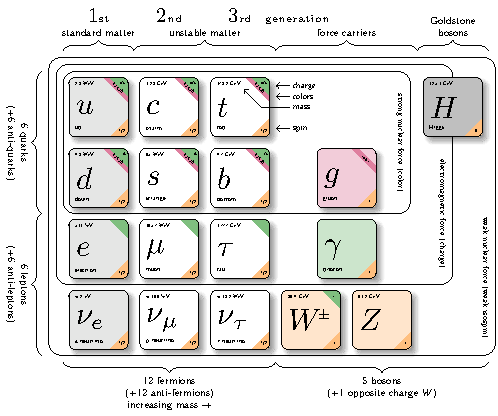
\includegraphics[width=0.84\mylength]{resources/SM_particles/SM_particles.pdf}
    \vspace*{-0.0cm}
    \caption{Elementary particles of the Standard Model. The electric charge, mass and spin of each particle are shown. Figure from Ref. \cite{Wongel:2816526}.}
    \label{fig:SM}
    \vspace*{-0.3cm}
\end{figure}
These three factors of the gauge symmetry group give rise to the three fundamental interactions between fermions, which are mediated by gauge bosons. To be precise, each generator of a local invariant gauge group induces a massless gauge boson. In the same way that in quantum electrodynamics (QED), the local gauge invariance of the theory under the $\text{U}(1)$ group leads to the existence of a massless gauge field $A_\mu$ (the photon field), in the SM, the process is analogous.

The invariance of the SM under $\text{SU}(3)_{\text{C}}$ postulates the existence of the gluon. More precisely, the eight generators of $\text{SU}(3)_{\text{C}}$ introduce eight gluons that mediate the strong force between particles that possess color charge (quarks and gluons). This is known as the quantum chromodynamics (QCD) sector of the Standard Model.

Similarly, the invariance of the second and third factors $\text{SU}(2)_{\text{L}}\times \text{U}(1)_{\text{Y}}$ indicates the existence of the photon, the $Z^{0}$ and the $W^{\pm}$ bosons. In this case, unlike in QED or QCD, we cannot directly associate the photon with the generator of the hypercharge group $\text{U}(1)_{\text{Y}}$ and the $Z^{0}$, $W^{\pm}$ bosons with the generators of the left weak isospin group $\text{SU}(2)_{\text{L}}$. Instead, the generators of $\text{SU}(2)_{\text{L}}\times \text{U}(1)_{\text{Y}}$ give rise to four intermediate vector bosons ($W_\mu^{1,2,3}$ for $\text{SU}(2)_{\text{L}}$ and $B_\mu$ for $\text{U}(1)_{\text{Y}}$), which are then mixed through the weak mixing angle or Weinberg angle, $\theta_{\text{W}}$, to produce the physical $\gamma$ ($A_\mu$), $Z^{0}$, $W^{\pm}$. The physical bosons are then defined as:
\begin{align*}
    W_\mu^{\pm} &= \frac{1}{\sqrt{2}}(W_\mu^{1}\mp iW_\mu^{2})\\
    \begin{pmatrix}
        A_\mu \\
        Z^{0}_\mu
    \end{pmatrix}
    &=
    \begin{pmatrix}
        \cos{\theta_{\text{W}}} & \sin{\theta_{\text{W}}} \\
        -\sin{\theta_{\text{W}}} & \cos{\theta_{\text{W}}}
    \end{pmatrix}
    \begin{pmatrix}
        B_\mu \\
        W^{3}_\mu
    \end{pmatrix}
\end{align*}
By the definition of the groups $\text{SU}(2)_{\text{L}}$ and $\text{U}(1)_{\text{Y}}$, the field $W_\mu^{1,2,3}$ couples only to left-handed (negative helicity) particles, whereas the hypercharge field $B_\mu$ couples to both left and right components with the same strength. Therefore, the intermediate boson mixing implies that $W^{\pm}$ only couple to left-handed particles, but $Z^{0}$ couples to both left and right-handed particles with different strengths, inducing (non-maximal) parity violation.

All gauge bosons that arise from the generators of gauge-invariant groups are expected to be massless; otherwise, the principle of local gauge invariance is spoiled and the theory becomes unrenormalizable. However, this contradicts experimental observations, which confirm that the $Z^{0}$ and $W^{\pm}$ bosons are, in fact, massive. This breaking of gauge invariance when giving a mass to a particle is not restricted only to gauge bosons but also happens for fermions. In the SM, to allow for massive fields, all particles obtain their masses using spontaneous symmetry breaking (SSB) via the Higgs mechanism.

Spontaneous symmetry breaking is a fundamental principle of QFT used to explain how gauge bosons (and, in general, massive particles) can acquire non-vanishing mass while maintaining the theory gauge-invariant. This process describes systems where the Lagrangian obeys symmetries, but the lowest-energy vacuum solutions do not exhibit the same symmetries. In the case of the Higgs mechanism, it relies on the existence of an $\text{SU}(2)$ doublet complex scalar field $\phi$ with hypercharge $Y = +1$, which can be written as 
\begin{equation*}
    \phi=
    \begin{pmatrix}
        \phi^{+} \\
        \phi^{0}
    \end{pmatrix}
\end{equation*}
with $(\phi^{+})^{*}=\phi^{-}$ and $(\phi^{0})^{*}=\phi^{0}$. This scalar field has a Lagrangian density given by $\mathcal{L}=\abs{D_{\mu}\phi}^2 - V(\phi)$ and a potential $V(\phi) = \mu^2\phi^\dag\phi+\lambda(\phi^\dag\phi)^2$, where $D_\mu$ is the covariant derivative determined by $\text{SU}(2)_{\text{L}}\times \text{U}(1)_{\text{Y}}$. When expanding the field $\phi$ around a minimum of the potential $V$, one finds out that there are infinitely many values of $\phi$ that minimize the potential. Suppose one expands $\phi$ around
\begin{equation*}
    \phi_{0}=\frac{1}{\sqrt{2}}
    \begin{pmatrix}
        0 \\
        v
    \end{pmatrix},\quad \text{so}\quad
    \phi(x)=\frac{1}{\sqrt{2}}
    \begin{pmatrix}
        0 \\
        v + h(x)
    \end{pmatrix}.
\end{equation*}
Deciding to expand the field around a chosen minimum $\phi_{0}$ spontaneously breaks the $\text{SU}(2)_{\text{L}}\times \text{U}(1)_{\text{Y}}$ symmetry, which in turn generates mass terms for the weak bosons in the Lagrangian. To convince oneself of the last implication it suffices to expand the $\abs{D_{\mu}\phi}^2$ term around the chosen vacuum expectation value $v$, which will produce terms of the form $M_{W}^2W_\mu^{+}W^{-\mu}$ and $M_{Z}^2Z_\mu^{0}Z^{0\mu}$ in the Lagrangian density. This scalar field is called the Higgs field.

With that, the Standard Model of particle physics is governed by the following Lagrangian density:
\begin{equation}
\begin{aligned}
    \mathcal{L}_{\text{SM}} &= -\frac{1}{4}G_{\mu\nu}^{a}G^{a\mu\nu} -\frac{1}{4}W_{\mu\nu}^{i}W^{i\mu\nu} -\frac{1}{4}B_{\mu\nu}B^{\mu\nu} \label{eq:L_SM}\\
    &+ \abs{D_\mu\phi}^2 - \mu^2\phi^\dag\phi - \lambda(\phi^\dag\phi)^2 \\
    &+ i\left[\bar{L}\slashed{D} L + \bar{e}\slashed{D} e + \bar{Q}\slashed{D} Q + \bar{u}\slashed{D} u + \bar{d}\slashed{D} d\right] \\
    & -\left[Y_{e}\bar{L}\phi e + Y_u\bar{Q}\phi^{c} u + Y_d\bar{Q}\phi d + \text{h.c.}\right]
\end{aligned}
\end{equation}
The used notation is the following: $\phi$, $Q$, $u$, $d$, $L$, $e$ are the SM Higgs, quarks and lepton fields. The left-handed doublets are denoted by capital letters as
\begin{equation*}
    Q_{i} = 
    \begin{pmatrix}
    u_{L}^{i}\\
    d_{L}^{i}
    \end{pmatrix}
    \text{ for quarks, and } L_{\alpha} = 
    \begin{pmatrix}
    \nu_{L}^{\alpha}\\
    e_{L}^{\alpha}
    \end{pmatrix}\text{for leptons,}
\end{equation*}
whereas for the right-handed singlets lowercase letters are used. We use the usual covariant derivative defined as
\begin{equation*}
    D_\mu = \partial_\mu - ig_{s}T^{a}G_\mu^{a} - ig\frac{\sigma^{i}}{2}W_\mu^{i} - ig'\frac{Y}{2}B_\mu
\end{equation*}
and where $T^{a}$, $\sigma^{i}$ (Pauli matrices) and $Y$ (weak hypercharge) are the generators of SU(3), SU(2) and SU(1) respectively, and $g_s$, $g$ and $g'$ are the coupling constants. $\phi^{c}$ is the charge conjugate of $\phi$ defined by $\phi^{c} = i\frac{\sigma_{2}}{2}\phi^{\dag}$.

The first line in Equation \eqref{eq:L_SM} describes the kinetic energies and interactions of the gauge boson fields. The field strength tensors associated to $G_\mu^{a}$ (gluons), $W_\mu^{i}$ and $B_\mu$ ($W^{\pm}$, $Z^{0}$, $\gamma$) are defined by
\begin{align*}
    G_{\mu\nu}^{a} &= \partial_\mu G_\nu^{a} - \partial_\nu G_\mu^{a} - g_{s} f^{abc}G_\mu^{b}G_\nu^{c}\\
    W_{\mu\nu}^{i} &= \partial_\mu W_\nu^{i} - \partial_\nu W_\mu^{i} - g \epsilon^{ijk}W_\mu^{j}W_\nu^{k}\\
    B_{\mu\nu} &= \partial_\mu B_\nu - \partial_\nu B_\mu
\end{align*}
where $f^{abc}$ and $\epsilon^{ijk}$ are the group structure constants of SU(3) and SU(2), respectively (the strength tensor of the hypercharge field $B_\mu$ does not have this extra term since U(1) is abelian). This is the origin of gluons and electroweak bosons self-interactions.

The second line in Equation \eqref{eq:L_SM} describes the Higgs field and generates the masses of the weak gauge bosons $W^{\pm}$, $Z^{0}$ and of the Higgs boson. In particular, the term $\abs{D_{\mu}\phi}^2$ generates all interactions between the gauge bosons and the Higgs field.

The third line in Equation \eqref{eq:L_SM} is responsible for fermion kinetic energies as well as their interactions with all bosons (gluons and eletroweak bosons). We have five terms: left-handed lepton doublets, right-handed lepton singlets (only charged leptons since right-handed neutrinos do not couple in the SM), left-handed quark doublets, right-handed up-type quark singlets and right-handed down-type quark singlets. The covariant derivative terms relative to each group apply only to these fermions that transform under that group. For instance, the first term would expand as
\begin{equation*}
    i\bar{L}\slashed{D} L = i\bar{L}\gamma^{\mu}D_\mu L = i
    \begin{pmatrix}
        \bar{\nu}_{L}^{\alpha} & \bar{e}_{L}^{\alpha}
    \end{pmatrix}
    \gamma^{\mu}\left(\partial_\mu - ig\frac{\sigma^{i}}{2}W_\mu^{i} - ig'\frac{Y}{2}B_\mu\right)
    \begin{pmatrix}
        \nu_{L}^{\alpha}\\
        e_{L}^{\alpha}
    \end{pmatrix},
\end{equation*}
since the leptons do not carry color charge, but the fourth term would expand as
\begin{equation*}
    i\bar{u}\slashed{D} u = i\bar{u}\gamma^{\mu}D_\mu u = i \bar{u}_{R}^{i}
    \gamma^{\mu}\left(\partial_\mu - ig_{s}T^{a}G_\mu^{a} - ig'\frac{Y}{2}B_\mu\right) u_{R}^{i},
\end{equation*}
because the right-handed quark is a singlet under SU(2)$_{\text{L}}$.

Finally, the couplings between the Higgs boson and the fermions, and in turn fermion masses, are generated by the fourth line in Equation \eqref{eq:L_SM}. These terms are gauge invariant, but give rise to fermion masses. For example, for the leptons and taking the Higgs field expansion around $\phi_0$, the first term will expand as
\begin{equation*}
    Y_{e}\bar{L}\phi e = \frac{Y_e^{\alpha\beta}}{\sqrt{2}}
    \begin{pmatrix}
        \bar{\nu}_{L}^{\alpha} & \bar{e}_{L}^{\alpha}
    \end{pmatrix}
    \begin{pmatrix}
        0\\
        v + h(x)
    \end{pmatrix}
    e_{R}^{\beta} = \frac{Y_e^{\alpha\beta}}{\sqrt{2}}\left[v + h(x)\right] \bar{e}_{L}^{\alpha}e_{R}^{\beta}
\end{equation*}
which in addition to its hermitian conjugate will ultimately yield the term
\begin{equation*}
    \frac{Y_e^{\alpha\beta}}{\sqrt{2}} v \left[\bar{e}_{L}^{\alpha}e_{R}^{\beta} + \bar{e}_{R}^{\alpha}e_{L}^{\beta}\right] = \frac{Y_e^{\alpha\beta}v}{\sqrt{2}} \bar{e}^{\alpha}e^{\beta}
\end{equation*}
after spontaneous symmetry breaking. One can easily identify the mass of the three charged leptons as
\begin{equation*}
    m_{e} = \frac{Y_e^{ee} v}{\sqrt{2}},\quad m_{\mu} = \frac{Y_e^{\mu\mu} v}{\sqrt{2}}\quad\text{and}\quad m_{\tau} = \frac{Y_e^{\tau\tau} v}{\sqrt{2}}.
\end{equation*}
To generate mass terms for up-type like quarks the Yukawa term involves the charge conjugate of the Higgs doublet (as in the second term of the fourth line in Equation \eqref{eq:L_SM}).

The Standard Model Lagrangian in Equation \eqref{eq:L_SM} governs the interactions between all particles within the theory. These interactions can be represented as vertices in Feynman diagrams. The vertices shown in Figure \ref{fig:SM_vertices} are all possible interactions in the SM, and are constructed from the terms in the SM Lagrangian. Terms that, after SSB, involve only two fields do not result in vertices as they are interpreted as mass terms. Consequently, we only see vertices with at least three fields.

For instance, to derive the QED vertex for the electron, one must expand the terms $i\left(\bar{L}\slashed{D} L + \bar{e}\slashed{D} e\right)$ and keep the terms of the form $\bar{e}\cdot\ldots\cdot e$. This expansion ultimately yields two contributions. The first one corresponds to the coupling of the electron to the photon field:
\begin{equation}
    \label{eq:qed_term}
    -\frac{gg'}{\sqrt{{g'}^2 + g^2}}\bar{e}\gamma^\mu eA_\mu = -e \bar{e}\gamma^\mu eA_\mu\ .
\end{equation}
The first $e$ in the latter expression refers to the electrical charge, therefore connecting both couplings $g$ and $g'$ with the electrical charge and the weak mixing angle, yielding $e=g'\cos{\theta_{\text{W}}}=g\sin{\theta_{\text{W}}}$. The second term that arises corresponds to the $Z^0$ boson:
\begin{equation*}
    \frac{1}{\sqrt{{g'}^2 + g^2}}\left(\frac{{g'}^2 - g^2}{2}\bar{e}_{L}\gamma^\mu e_{L} + {g'}^2 \bar{e}_{R}\gamma^\mu e_{R}\right)Z^0_\mu \ .
\end{equation*}
We can see that the $Z^0$ couples to both left-handed and right-handed components of the electron but with different strengths. Hence, by removing the fields from Equation \eqref{eq:qed_term} and multiplying by $i$, the coupling of the electron to the photon associated with the QED vertex is
\begin{equation}
    \label{eq:qed_vertex}
\vcenter{\hbox{
\setlength{\mylength}{\textwidth}
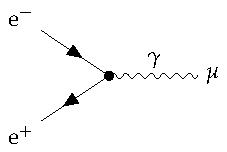
\includegraphics[height=0.16\mylength]{resources/SM_vertices/qed.pdf}
 }} = -ie \gamma^\mu \ .
\end{equation}
Each of the vertices in Figure \ref{fig:SM_vertices} has an associated factor that can be computed from the SM Lagrangian density in a similar manner. Therefore, we can observe, for example, that the Higgs boson does not couple to the photon or the gluon field, and that there is no direct interaction between three fermions.

\begin{figure}[!ht]
    \captionsetup[subfigure]{labelformat=empty}
    \vspace*{-0.2cm}
    \centering
    \setlength{\mylength}{\textwidth}
    \begin{subfigure}[t]{0.33\mylength}
            \centering
            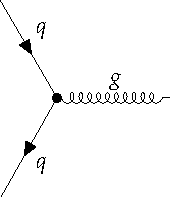
\includegraphics[height=0.20\mylength]{resources/SM_vertices/v1.pdf}
            \setlength{\unitlength}{0.25\mylength}
            %\caption{\footnotesize (a)}
    \end{subfigure}%
    \begin{subfigure}[t]{0.33\mylength}
            \centering
            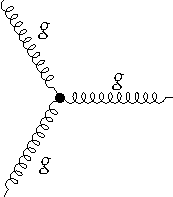
\includegraphics[height=0.20\mylength]{resources/SM_vertices/v2.pdf}
            \setlength{\unitlength}{0.25\mylength}
            %\caption{\footnotesize (b)}
    \end{subfigure}%
    \begin{subfigure}[t]{0.33\mylength}
            \centering
            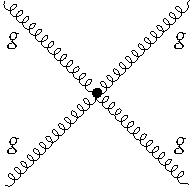
\includegraphics[height=0.20\mylength]{resources/SM_vertices/v3.pdf}
            \setlength{\unitlength}{0.25\mylength}
            %\caption{\footnotesize (c)}
    \end{subfigure}%\begin{subfigure}[t]{0.33\mylength}\baselineskip    
    \vskip\baselineskip
    \vspace*{-0.1cm}
    \begin{subfigure}[t]{0.33\mylength}
            \centering
            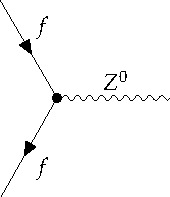
\includegraphics[height=0.20\mylength]{resources/SM_vertices/v4.pdf}
            \setlength{\unitlength}{0.25\mylength}
            %\caption{\footnotesize (d)}
    \end{subfigure}%\begin{subfigure}[t]{0.33\mylength}
    \begin{subfigure}[t]{0.33\mylength}
            \centering
            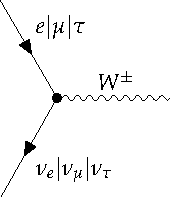
\includegraphics[height=0.20\mylength]{resources/SM_vertices/v5.pdf}
            \setlength{\unitlength}{0.25\mylength}
            %\caption{\footnotesize (e)}
    \end{subfigure}%\begin{subfigure}[t]{0.33\mylength}
    \begin{subfigure}[t]{0.33\mylength}
            \centering
            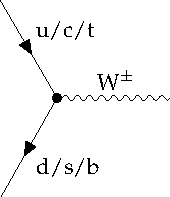
\includegraphics[height=0.20\mylength]{resources/SM_vertices/v6.pdf}
            \setlength{\unitlength}{0.25\mylength}
            %\caption{\footnotesize (f)}
    \end{subfigure}%
    \vskip\baselineskip
    \vspace*{-0.1cm}
    \begin{subfigure}[t]{0.33\mylength}
            \centering
            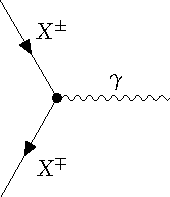
\includegraphics[height=0.20\mylength]{resources/SM_vertices/v7.pdf}
            \setlength{\unitlength}{0.25\mylength}
            %\caption{\footnotesize (g)}
    \end{subfigure}%\begin{subfigure}[t]{0.33\mylength}
    \begin{subfigure}[t]{0.33\mylength}
            \centering
            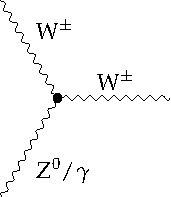
\includegraphics[height=0.20\mylength]{resources/SM_vertices/v8.pdf}
            \setlength{\unitlength}{0.25\mylength}
            %\caption{\footnotesize (h)}
    \end{subfigure}%\begin{subfigure}[t]{0.33\mylength}
    \begin{subfigure}[t]{0.33\mylength}
            \centering
            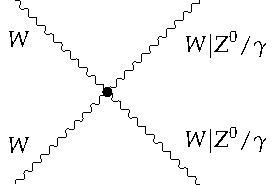
\includegraphics[height=0.20\mylength]{resources/SM_vertices/v9.pdf}
            \setlength{\unitlength}{0.25\mylength}
            %\caption{\footnotesize (i)}
    \end{subfigure}%
    \vskip\baselineskip
    \vspace*{-0.1cm}
    \begin{subfigure}[t]{0.33\mylength}
            \centering
            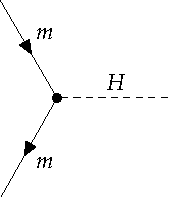
\includegraphics[height=0.20\mylength]{resources/SM_vertices/v10.pdf}
            \setlength{\unitlength}{0.25\mylength}
            %\caption{\footnotesize (j)}
    \end{subfigure}%\begin{subfigure}[t]{0.33\mylength}
    \begin{subfigure}[t]{0.33\mylength}
            \centering
            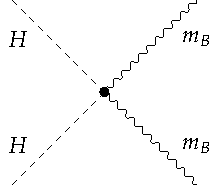
\includegraphics[height=0.20\mylength]{resources/SM_vertices/v11.pdf}
            \setlength{\unitlength}{0.25\mylength}
            %\caption{\footnotesize (k)}
    \end{subfigure}%\begin{subfigure}[t]{0.33\mylength}
    \vspace*{-0.0cm}
    \caption{All possible interactions in the Standard Model, represented by Feynman diagrams. $q$ is any quark, $g$ is (any) gluon, $X^{\pm}$ is any charged particle, $\gamma$ is a photon, $f$ is any fermion, $m$ is any massive particle (except neutrinos), $m_{B}$ is any massive boson. In diagrams with multiple particle labels separated by / one particle label is chosen. In diagrams with particle labels separated by | the labels must be chosen in the same order. For example, in the four electroweak boson case the valid diagrams are $WWWW$, $WWZZ$, $WW\gamma\gamma$ and $WWZ\gamma$.}
    \label{fig:SM_vertices}
    \vspace*{-0.2cm}
\end{figure}

The Standard Model has proven to predict numerous measurements with exceptional precision. Yet, the theory does not explain why the masses of all particles are given by the values we measure. In fact, aside from the mass of the photon, which is protected by the unbroken U(1) gauge symmetry of QED, the SM does not predict any other mass value. All fermion masses (or equivalently, the Yukawa couplings) are free parameters of the theory.

While this theory has been remarkably successful, it cannot serve as the final theory of nature, as numerous unresolved puzzles persist. Many cosmological observations remain unaccounted for by the SM, such as the baryon-antibaryon asymmetry, the behaviour of gravity as described by General Relativity, the accelerated expansion of the Universe — potentially described by dark energy — and the absence of a suitable candidate for dark matter. Furthermore, the SM fails to explain the non-vanishing mass of the neutrinos as a consequence of neutrino flavour oscillation. In pursuit of a superior theory capable of encompassing the SM as well as these (and many other) discrepancies, the physics community is thoroughly trying to ``break'' the Standard Model to unveil hints towards an ultimate theory.

\section{The Higgs boson}\label{sec:Higgs_boson}

In 1964, Peter Higgs, along with five other theoretical physicists, proposed the Higgs mechanism to explain how certain particles (fermions and weak bosons) might acquire mass in local gauge theories \cite{Higgs:1964pj,Englert:1964et,Guralnik:1964eu}. If these ideas were correct, a spin-0 particle (namely the Higgs boson) should exist and possess some well-defined properties. Nearly 50 years later, on the 4\textsuperscript{th} of July 2012, a scalar particle consistent with the Higgs boson was discovered at the LHC by the CMS and ATLAS collaborations \cite{CMS:2012qbp,ATLAS:2012yve}.

\subsection{Properties of the Higgs boson}

The Higgs boson is a weak isospin SU(2)$_{\text{L}}$ doublet, massive scalar neutral boson. Table \ref{tab:higgs_properties} summarizes the SM predicted properties \cite{Djouadi:2005gi, LHCHiggsCrossSectionWorkingGroup:2016ypw} as well as the measured properties of the Higgs boson from the Particle Data Group (PDG) \cite{PDG}.

\begin{table}[ht]
    \centering
    \begin{tabular}{|l|l|l|}
        \hline
        \cellcolor{lightgray}Property & \cellcolor{lightgray}SM prediction & \cellcolor{lightgray}Mesasured value \\ \hline
        Mass                & $m \lesssim 700 \;\; \text{GeV}$ & $m = 125.25 \pm 0.17 \;\; \text{GeV}$             \\
        Spin                &  $J=0$ & $J=0$                                             \\
        Electric charge     & $q=0$  & $q=0$                                             \\
        Full width          & $\Gamma = 4.12 \pm 0.06 \;\;  \text{MeV}$  & $\Gamma = 3.2^{+2.8}_{-2.2} \;\;  \text{MeV}$     \\
        Lifetime            & $\tau = (1.60 \pm 0.02) \times 10^{-22} \;\;  \text{s}$  & $\tau = 2.1^{+4.5}_{-1.0} \times 10^{-22} \;\;  \text{s}$   \\ \hline
    \end{tabular}
    \caption{Properties of the Higgs boson. The SM prediction for the full width and the lifetime depend on the Higgs mass, which is assumed to be $m = 125.25$ GeV.}
    \label{tab:higgs_properties}
\end{table}

As stated previously, the SM does not predict the mass of any particle (except for the photon), including the mass of the Higgs boson. Nevertheless, some theoretical arguments, such as radiative corrections and unitarity considerations, enabled theorists to establish upper bounds on the Higgs mass \cite{Djouadi:2005gi}.

\subsection{Main production modes of the Higgs boson}\label{subsec:higgs_production}

To understand the production and decay modes of the Higgs boson, it's important to recall that the Higgs boson couples to all the other massive particles of the SM (it couples to the gauge bosons via the $\abs{D_{\mu}\phi}^2$ term in the Higgs part of the SM Lagrangian and to fermions via the Yukawa couplings), as well as to itself. Expanding the terms in the Lagrangian reveals that the coupling between the Higgs boson and any fermion is directly proportional to the particle's rest mass, while the coupling between the Higgs boson and any massive vector boson is directly proportional to the square of the particle's rest mass.

Collecting the relevant Feynman vertices, one can determine the dominant production modes for the Higgs boson, as shown in Figure \ref{fig:Higgs_production}. Since the heavier the particle, the stronger its Higgs coupling constant is, we observe that in most cases, the particles involved in the vertex where the Higgs boson is produced are very heavy (top and bottom quarks and massive gauge bosons).

\begin{figure}[!ht]
    \captionsetup[subfigure]{labelformat=empty}
    \vspace*{-0.2cm}
    \centering
    \setlength{\mylength}{\textwidth}
    \begin{subfigure}[t]{0.33\mylength}
            \centering
            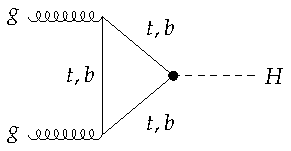
\includegraphics[height=0.16\mylength]{resources/H_production_diagrams/v1.pdf}
            \setlength{\unitlength}{0.25\mylength}
            \caption{\footnotesize (a)}
    \end{subfigure}%
    \begin{subfigure}[t]{0.33\mylength}
            \centering
            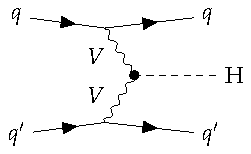
\includegraphics[height=0.16\mylength]{resources/H_production_diagrams/v2.pdf}
            \setlength{\unitlength}{0.25\mylength}
            \caption{\footnotesize (b)}
    \end{subfigure}%
    \begin{subfigure}[t]{0.33\mylength}
            \centering
            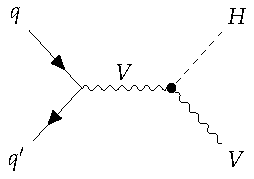
\includegraphics[height=0.185\mylength]{resources/H_production_diagrams/v3.pdf}
            \setlength{\unitlength}{0.25\mylength}
            \caption{\footnotesize (c)}
    \end{subfigure}%\begin{subfigure}[t]{0.33\mylength}\baselineskip    
    \vskip\baselineskip
    \vspace*{-0.1cm}
    \begin{subfigure}[t]{0.33\mylength}
            \centering
            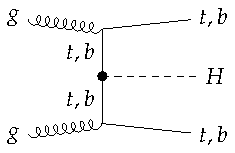
\includegraphics[height=0.16\mylength]{resources/H_production_diagrams/v4.pdf}
            \setlength{\unitlength}{0.25\mylength}
            \caption{\footnotesize (d)}
    \end{subfigure}%\begin{subfigure}[t]{0.33\mylength}
    \begin{subfigure}[t]{0.33\mylength}
            \centering
            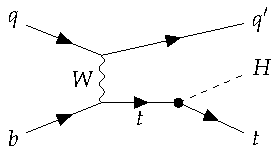
\includegraphics[height=0.16\mylength]{resources/H_production_diagrams/v5.pdf}
            \setlength{\unitlength}{0.25\mylength}
            \caption{\footnotesize (e)}
    \end{subfigure}%\begin{subfigure}[t]{0.33\mylength}
    \begin{subfigure}[t]{0.33\mylength}
            \centering
            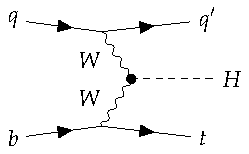
\includegraphics[height=0.16\mylength]{resources/H_production_diagrams/v6.pdf}
            \setlength{\unitlength}{0.25\mylength}
            \caption{\footnotesize (f)}
    \end{subfigure}%
    \vspace*{-0.0cm}
    \caption{Higgs boson production in (a) gluon-gluon fusion (ggH), (b) vector boson fusion (VBF), (c) associated production with a $W$ or $Z$ (V) boson (VH), also known as Higgsstrahlung, (d) associated production with a top or bottom quark pair (ttH or bbH), or tt fusion, and (e, f) associated production with a single top quark (tH).}
    \label{fig:Higgs_production}
    \vspace*{-0.0cm}
\end{figure}

Despite being a second-order process (it requires a heavy quark loop), the strong coupling to heavy quarks makes gluon fusion the process that contributes the most to the production of the Higgs boson at the LHC, a proton-proton (pp) collider. The LHC is a gluon-gluon collider when it comes to Higgs production, as gluons dominate the production of Higgs bosons with a mass of around 125 GeV. The second most important process at the LHC is vector boson fusion, where two fermions collide and exchange a virtual vector boson, which radiates a Higgs boson. The third contribution to Higgs boson production, and the first one at LEP, is associated production with a vector boson or Higgsstrahlung. In this production mode, a fermion and antifermion collide and can form a virtual $W^{\pm}$ or $Z^0$ boson which, if it carries enough energy, can emit a Higgs boson.

\todo{Add Higgs production signatures}

To compare the different production cross sections with the SM predictions, we introduce some important quantities to describe interactions at particle colliders. The \textit{center-of-mass energy} $\sqrt{s}$ describes the combined energy of the collided particle beams and is defined as the square root of the Mandelstam variable
\begin{equation*}
\sqrt{s} = \sqrt{(p_1+p_2)^2}\ ,
\end{equation*}
where $p_1$ and $p_2$ are the four-momenta of the two particles. When colliding elementary particles (e.g., $e^+e^-$), the center-of-mass energy is precisely the available energy to produce particles in the collision. When colliding composite particles (e.g., protons), however, the available energy to produce particles is slightly less due to the parton distribution functions within the proton, and there is an energy spread. The \textit{cross section} $\sigma$ of a process describes the likelihood of a specific final state, as a measure of the effective area or target size for a particular interaction. It is measured in units of area, usually barns, defined as barn $= 10^{-28}$ cm$^{2}$. The number of events per unit time can be expressed in terms of the \textit{instantaneous luminosity} $\mathscr{L}$ and the cross section of the studied event $\sigma$ as
\begin{equation*}
    \frac{\d N_{\text{events}}}{\d t} = \mathscr{L}\sigma\ ,
\end{equation*}
and the \textit{integrated luminosity} is defined as 
\begin{equation*}
    L = \int\mathscr{L}\d t\ .
\end{equation*}
Finally, the \textit{signal strength} $\mu$ expresses a measured cross section divided by the expected SM value.

Having established these fundamental concepts, we can now compare the theoretical and measured cross sections for the production of the Higgs boson. Our analysis uses 2018 data from the LHC, with a center-of-mass energy of $\sqrt{s} = 13$ TeV and an integrated luminosity of $L=39.54$ fb$^{-1}$. According to the SM and assuming $m_H = 125.25\ \GeV$, the total Higgs boson cross section at a center-of-mass energy of $\sqrt{s} = 13$ TeV is $\sigma = 55500 \pm 2800$ fb \cite{LHCHiggsCrossSectionWorkingGroup:2016ypw}, with around 87\% coming from gluon fusion, 7\% from vector boson fusion and 4\% from Higgsstrahlung. The predicted and measured cross section of the Higgs boson at $\sqrt{s} = 13$ TeV from different production modes are shown in Table \ref{tab:Higgs_production}.

\begin{table}[ht]
    \centering
    \begin{tabular}{|l|c|c|c|}
        \hline
        \multicolumn{1}{|c|}{\cellcolor{lightgray}Production mode} & \cellcolor{lightgray} SM $\sigma$ [fb] & \cellcolor{lightgray} Measured $\sigma$ [fb] & \cellcolor{lightgray} Measured $\mu$ \\ \hline
        ggH                         & $48400 \pm 2440$          & $47000 \pm 4500$          & $0.97 \pm 0.08$           \\
        VBF                         & $3774 \pm 81$             & $3020 \pm 460$            & $0.80 \pm 0.12$    \\
        WH                          & $1365  \pm 28$            & $2030  \pm 360$           & $1.49 \pm 0.26$     \\
        %W$^+$H ($W^+\to l^+\nu$)    & $3\times(93.7  \pm 1.8)$  & $0.0  \pm 0.0$        \\
        %W$^+$H                      & $835  \pm 17$             & $0.0  \pm 0.0$        \\
        %W$^-$H ($W^-\to l^-\nu$)    & $3\times(59.4  \pm 1.2)$  & $0.0  \pm 0.0$        \\
        %W$^-$H                      & $530  \pm 11$             & $0.0  \pm 0.0$        \\
        Z$^0$H                      & $879  \pm 36$             & $1130  \pm 220$           & $1.29 \pm 0.24$    \\
        %Z$^0$H ($Z^0\to l^-l^+$)    & $3\times(29.7  \pm 1.2)$  & $0.0  \pm 0.0$        \\
        %ggZ$^0$H ($Z^0\to l^-l^+$)  & $3\times(93.7  \pm 1.8)$  & $0.0  \pm 0.0$        \\
        %Z$^0$H ($Z^0\to \nu\bar{\nu}$)& $3\times(177  \pm 7)$  & $0.0  \pm 0.0$        \\
        %ggZ$^0$H ($Z^0\to \nu\nu$)  & $3\times(93.7  \pm 1.8)$  & $0.0  \pm 0.0$        \\
        ttH + H                     & $582  \pm 61$             & $660  \pm 130$             & $1.13 \pm 0.18$    \\
        %ttH                        & $505  \pm 50$            & $0.0  \pm 0.0$        \\
        bbH                         & $484  \pm 116$            & -       & - \\ \hline
        %tH + tbarH (s and t channels)                  & $77  \pm 12$            & $0.0  \pm 0.0$        \\ \hline
    \end{tabular}
    \caption{Cross section of the Higgs boson's most frequent production modes at $\sqrt{s} = 13$ TeV. SM values from Ref. \cite{LHCHiggsCrossSectionWorkingGroup:2016ypw}, measured $\mu$ values from Ref. \cite{CMS:2022dwd}, and measured $\sigma$ from $\sigma=\mu\sigma_{\text{SM}}$. At the moment of this writing, the bbH production channel has not been measured yet.}
    \label{tab:Higgs_production}
\end{table}

Since the most significant Higgs boson production channel is gluon fusion, within the limited timeframe of this project, our primary focus will be on this production mode. However, other modes, such as vector boson fusion or associated production with a $W$/$Z$ boson, share reasonable similarities with ggH in terms of implementation and could be further extensions of this analysis.

\subsection{Main decay channels of the Higgs boson}

The Higgs boson is a very short-lived particle, decaying almost instantaneously after its production into lighter particles. According to the couplings of the Higgs field to all other SM particles, at the first loop order, the Higgs boson predominantly decays to the most massive particles that are kinematically accessible. However, there are certain decay modes where the Higgs boson decays into massless particles, such as gluon or photon pairs, as the first-loop contributions are not negligible. Figure \ref{fig:Higgs_decays} shows the most relevant Feynman diagrams for the Higgs boson decay, while Table \ref{tab:Higgs_decays} presents the most frequent decay channels for the Higgs boson, comparing the SM predicted value to the measured value for every decay mode.

\begin{figure}[!ht]
    \captionsetup[subfigure]{labelformat=empty}
    \vspace*{-0.2cm}
    \centering
    \setlength{\mylength}{\textwidth}
    \begin{subfigure}[t]{0.5\mylength}
            \centering
            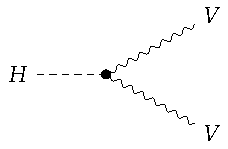
\includegraphics[height=0.1539\mylength]{resources/H_decay_diagrams/v1.pdf}
            \setlength{\unitlength}{0.25\mylength}
            \caption{\footnotesize (a)}
    \end{subfigure}%
    \begin{subfigure}[t]{0.5\mylength}
            \centering
            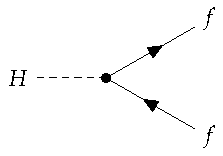
\includegraphics[height=0.1539\mylength]{resources/H_decay_diagrams/v2.pdf}
            \setlength{\unitlength}{0.25\mylength}
            \caption{\footnotesize (b)}
    \end{subfigure}%
    \vskip\baselineskip
    \vspace*{-0.1cm}
    \begin{subfigure}[t]{0.33\mylength}
            \centering
            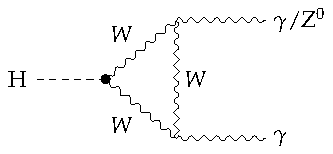
\includegraphics[height=0.1539\mylength]{resources/H_decay_diagrams/v3.pdf}
            \setlength{\unitlength}{0.25\mylength}
            \caption{\footnotesize (c)}
    \end{subfigure}%\begin{subfigure}[t]{0.5\mylength}
    \begin{subfigure}[t]{0.33\mylength}
            \centering
            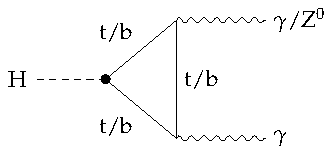
\includegraphics[height=0.1539\mylength]{resources/H_decay_diagrams/v4.pdf}
            \setlength{\unitlength}{0.25\mylength}
            \caption{\footnotesize (d)}
    \end{subfigure}%\begin{subfigure}[t]{0.5\mylength}
    \begin{subfigure}[t]{0.33\mylength}
            \centering
            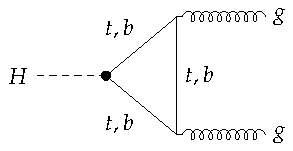
\includegraphics[height=0.1539\mylength]{resources/H_decay_diagrams/v5.pdf}
            \setlength{\unitlength}{0.25\mylength}
            \caption{\footnotesize (e)}
    \end{subfigure}%\begin{subfigure}[t]{0.5\mylength}
    \vspace*{-0.0cm}
    \caption{Higgs boson decays into (a) heavy vector boson pairs ($V$ is $Z^{0}/W^{\pm}$), (b) fermion-antifermion pairs, (c, d) photon pairs or $Z^0\gamma$, and (e) gluon pairs.}
    \label{fig:Higgs_decays}
    \vspace*{-0.0cm}
\end{figure}

\begin{table}[!ht]
    \centering
    \begin{tabular}{|l|c|c|cc|}
        \hline
        \multicolumn{1}{|c|}{\cellcolor{lightgray}Decay channel} & \cellcolor{lightgray} SM $\mathcal{B}$ (\%) & \cellcolor{lightgray} Measured $\mathcal{B}$ (\%) & \multicolumn{2}{c|}{\cellcolor{lightgray} Measured $\mu$} \\ \hline
        $\text{H}\decaysto b\bar{b}$     & $57.8 \pm 0.7$        & $60 \pm 12$         & $1.04 \pm 0.20$ & \cite{CMS:2018nsn}  \\
        $\text{H}\decaysto WW^*$         & $21.8 \pm 0.3$        & $20.7 \pm 2.1$      & $0.95 \pm 0.09$ & \cite{CMS:2022uhn}  \\
        $\text{H}\decaysto gg$           & $8.2 \pm 0.4$         & -                   & \multicolumn{2}{c|}{-}                \\
        $\text{H}\decaysto \tau^+\tau^-$ & $6.23 \pm 0.10$       & $6.1 \pm 1.1$       & $0.98 \pm 0.18$ & \cite{CMS:2017zyp}  \\
        $\text{H}\decaysto c\bar{c}$     & $2.87 \pm 0.16$       & $<40$               & $<14$ & \cite{CMS:2022psv}            \\
        $\text{H}\decaysto ZZ^*$         & $2.68 \pm 0.04$       & $2.6 \pm 0.3$       & $0.97 \pm 0.12$ & \cite{CMS:2022dwd}  \\
        $\text{H}\decaysto \gamma\gamma$ & $0.227 \pm 0.005$     & $0.254 \pm 0.021$   & $1.12 \pm 0.09$ & \cite{CMS:2021kom}  \\
        $\text{H}\decaysto Z\gamma$      & $0.155 \pm 0.009$     & $0.37 \pm 0.14$     & $2.4 \pm 0.9$ & \cite{CMS:2022ahq}    \\
        $\text{H}\decaysto s\bar{s}$     & $0.025 \pm 0.001$     & -                   & \multicolumn{2}{c|}{-}                \\
        $\text{H}\decaysto \mu^+\mu^-$   & $0.0216 \pm 0.0004$   & $0.026 \pm 0.009$   & $1.19 \pm 0.43$ & \cite{CMS:2020xwi}  \\ \hline
    \end{tabular}
    \caption{Most frequent decay modes of the Higgs boson. SM values from Ref. \cite{LHCHiggsCrossSectionWorkingGroup:2016ypw, CMS:2022dwd}, and measured $\mathcal{B}$ from $\mathcal{B}=\mu\mathcal{B}_{\text{SM}}$. At the moment of this writing, the $\text{H}\protect\decaysto gg$ and $\text{H}\protect\decaysto s\bar{s}$ decay channels have not been measured yet.}
    \label{tab:Higgs_decays}
\end{table}

The predicted values by the SM in Table \ref{tab:Higgs_decays} are of significant interest, and there are some remarks worth mentioning.

Firstly, it is observed that there is no decay $\text{H}\decaysto t\bar{t}$. This is because the Higgs boson is lighter than the top quark, $M_H = 125$ GeV < $m_t = 173$ Gev, making it not massive enough to produce a top-antitop quark pair. In fact, the Higgs boson can not even create one real top quark and one virtual top quark. Consequently, the presence of top quarks in the Higgs boson decays is limited to virtual loops, as the ones present in diagrams (d) and (e) of Figure \ref{fig:Higgs_decays}.

Let us examine the branching ratios in Table \ref{tab:Higgs_decays} more closely, starting with the fermionic decays. The Higgs-fermion vertex has a factor of
\begin{equation}
    \label{eq:higgs_fermion_vertex}
\vcenter{\hbox{
\setlength{\mylength}{\textwidth}
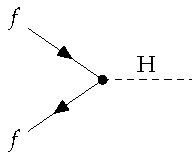
\includegraphics[height=0.16\mylength]{resources/SM_vertices/higgs_fermion.pdf}
 }} = -i \frac{m_f}{v} \ ,
\end{equation}
thus at first approximation, the expected decay width at tree level can be estimated as proportional to
\begin{equation}
\label{eq:Higgs_approx_fermions}
\Gamma(H\decaysto f\bar{f}) \propto N_C m_f^2 \ ,
\end{equation}
where $N_C$ is the number of colours (3 for quarks, 1 for leptons). It is important to note that the mass to use in the above expression is the \textit{running mass} of the particle at an energy scale of $\mu=M_{H}$, rather than the ones presented in Figure \ref{fig:SM}\footnote{The masses of the quarks that are typically provided, for example, in Ref. \cite{PDG}, are $m_u(\mu = 2\ \GeV)$, $m_d(\mu = 2\ \GeV)$, $m_s(\mu = 2\ \GeV)$, $m_c(\mu = m_c)$, $m_b(\mu = m_b)$. The $t$-quark mass is determined from event kinematics, see Ref. \cite{PDG}. The differences in the masses at the Higgs energy scale compared to the ``usual'' values are more pronounced for heavy quarks. For more information on running masses refer to Ref. \cite{Huang:2020hdv}.}. Using the running masses of the particles (for precise values of the running masses, see Ref. \cite{Huang:2020hdv}) and the approximation presented above, we obtain the following relation of decay widths for the quarks, taking $\Gamma(H\decaysto s\bar{s}) = 1$:
\begin{equation*}
    \Gamma(H\decaysto b\bar{b}):\Gamma(H\decaysto c\bar{c}):\Gamma(H\decaysto s\bar{s}) \approx  2834:136:1\ ,
\end{equation*}
while the full SM computation yields
\begin{equation*}
    \Gamma(H\decaysto b\bar{b}):\Gamma(H\decaysto c\bar{c}):\Gamma(H\decaysto s\bar{s}) =  2312:115:1\ .
\end{equation*}
The approximation in Equation \eqref{eq:Higgs_approx_fermions} is even better for leptons:
\begin{equation*}
    \Gamma(H\decaysto \tau^+\tau^-):\Gamma(H\decaysto \mu^+\mu^-) \approx  288.53:1\ ,
\end{equation*}
while the full SM computation is remarkably close, giving
\begin{equation*}
    \Gamma(H\decaysto \tau^+\tau^-):\Gamma(H\decaysto \mu^+\mu^-) =  288.43:1\ .
\end{equation*}
The discrepancies between this initial approximation and the results from the SM in Table \ref{tab:Higgs_decays} arise from phase space factors, higher-order Feynman diagrams, and, in the case of quarks, QCD corrections.

For vector bosons, the vertex has a factor of
\begin{equation}
    \label{eq:higgs_boson_vertex}
\vcenter{\hbox{
\setlength{\mylength}{\textwidth}
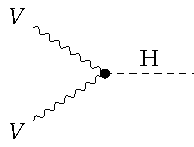
\includegraphics[height=0.16\mylength]{resources/SM_vertices/higgs_boson.pdf}
 }} = 2i \frac{M_V^2}{v}g^{\mu\nu} \ ,
\end{equation}
and similarly, one can estimate the expected decay width at tree level as proportional to
\begin{equation}
    \label{eq:Higgs_approx_bosons}
\Gamma(H\decaysto VV) \propto M_V^4 \ .
\end{equation}
When we compute the same relations as for the fermions we obtain
\begin{equation*}
    \Gamma(H\decaysto WW^*):\Gamma(H\decaysto ZZ^*) \approx  0.604:1\ ,
\end{equation*}
while the full SM computation differs by almost a factor of 14:
\begin{equation*}
    \Gamma(H\decaysto WW^*):\Gamma(H\decaysto ZZ^*) =  8.134:1\ .
\end{equation*}
Despite the vertex in Equation \eqref{eq:higgs_boson_vertex} suggesting that $\Gamma(H\decaysto WW^*) < \Gamma(H\decaysto ZZ^*)$ due to $M_W < M_Z$, other factors play a more significant role in the decay width than just the vertex factors in the boson decays. First of all, the phase space of the decay into $Z^0$ bosons includes an extra $\frac{1}{2}$ symmetry factor due to the decay involving two identical particles. The remaining factor of 7 arises from the inclusion of higher-order Feynman diagrams and, most significantly, from the phase space contribution. The latter contribution quantifies the number of valid momentum and energy configurations for the outgoing particles while still obeying the conservation of energy and momentum.

Note that $2M_W, 2M_Z > M_H > M_W, M_Z$, so for the Higgs boson to decay into two electroweak bosons, one of them must be \textit{off-shell} or \textit{virtual} (that is why one of them is marked with an asterisk). Off-shell or virtual particles do not need to satisfy the equation $E^2-p^2=m^2$, and are very short-lived. Therefore, for instance, the decay $H\decaysto WW^*$ means that the Higgs boson decays into a real $W$ boson and a virtual $W^*$ boson, which immediately decays into other particles. The phase factor for such a decay is intricate, as it involves the decay of a virtual boson into all possible channels, but is much smaller than it would be if the Higgs could decay to two real $Z^0$ or $W^{\pm}$ bosons. Additionally, the phase space contribution for the $ZZ^*$ channel is much smaller than that for the $WW^*$. This is mainly because the invariant mass of the virtual $Z^0$ boson tends to deviate more from the real $Z^0$ mass than the virtual $W^{\pm}$ boson is from the real $W^{\pm}$ mass.

There are two decaying channels in Table \ref{tab:Higgs_decays} that have not yet been experimentally tested. The $\text{H}\decaysto s\bar{s}$ channel is extremely challenging to measure due to its low branching fraction, which is more than two orders of magnitude smaller than that of the $c\bar{c}$ channel, for which only an upper bound is currently known. The other channel, accounting for approximately 8\% of the Higgs boson decays, is the decay into a pair of gluons. Experimentally determining this branching ratio at the LHC is incredibly difficult because it involves QCD processes that are almost indistinguishable from the QCD background present at the Large Hadron Collider.

Additionally, the Higgs boson decays into massless particles (gluons and photons) account for one in 12 decays. This indicates that, despite being higher-order Feynman diagrams, heavy quark loops, mainly involving top and bottom quarks, are not negligible and compete with tree-level decays. The decay into a pair of photons is particularly interesting because its signature in hadron colliders is relatively clean compared to the hadronic background, and was used in the Higgs boson discovery at the LHC in 2012.

\section{Searching of a model beyond the SM}\label{sec:BSM}

If the Standard Model is correct, the coupling between the Higgs boson and each massive fermion (boson) is directly proportional to the fermion's mass (the square of the boson's mass), as shown in Equations \eqref{eq:higgs_fermion_vertex} and \eqref{eq:higgs_boson_vertex}. One can visualize these relationships by plotting the Higgs couplings against the masses of the particles. According to the SM, this should result in a linear relationship, as in Figure \ref{fig:Yukawa_couplings}.

\begin{figure}[!ht]
    \vspace*{-0.0cm}
    \centering
    \setlength{\mylength}{\textwidth}
    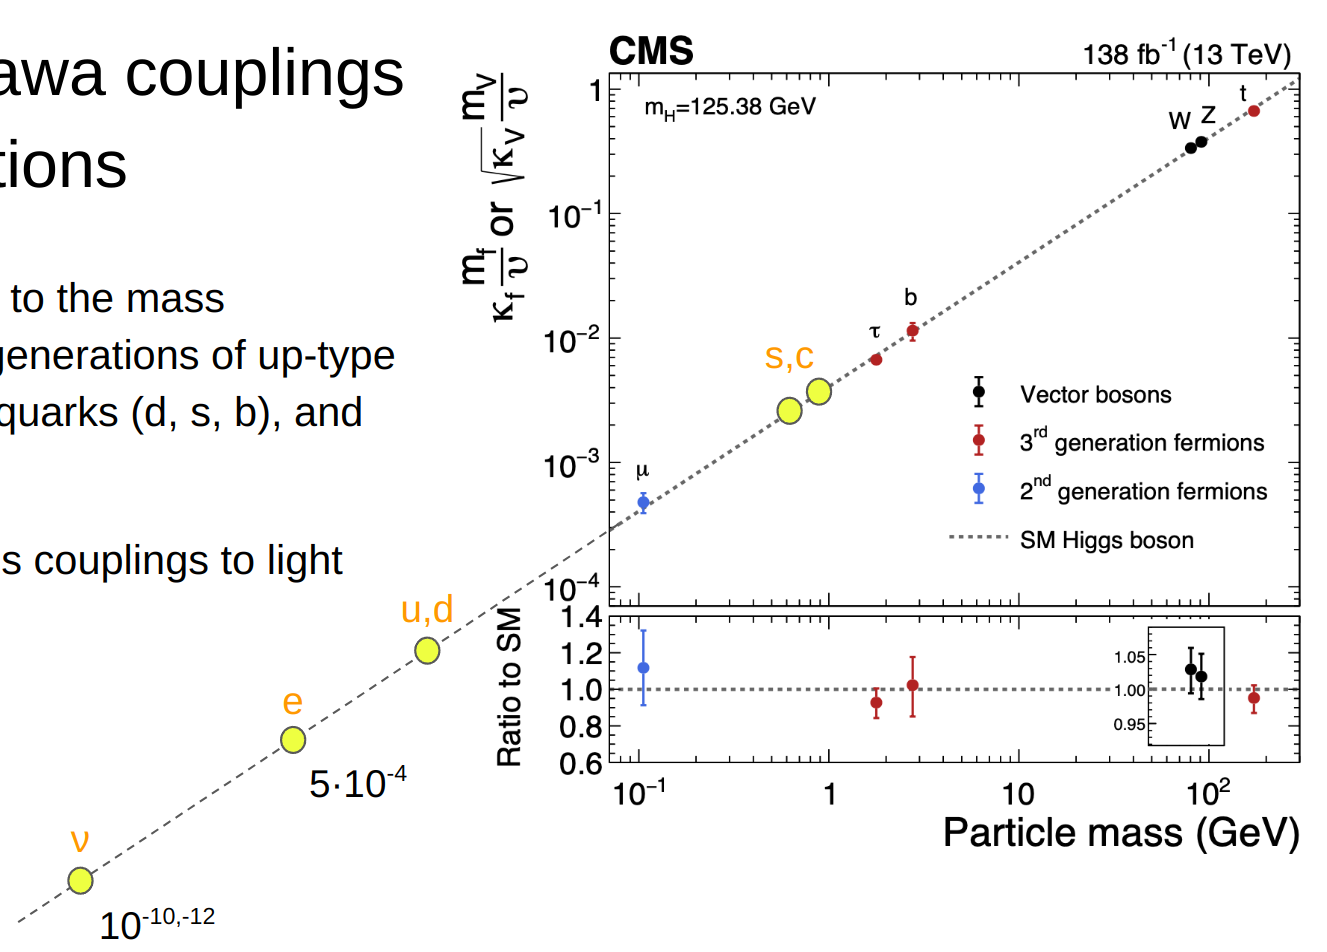
\includegraphics[width=0.60\mylength]{resources/Yukawa_couplings.png}
    \vspace*{-0.0cm}
    \caption{Relationship between the Yukawa couplings of the third-generation fermions, massive bosons, and the second-generation muon and its masses, from Ref. \cite{CMS:2022dwd}. The dashed straight line represents the Standard Model prediction.}
    \label{fig:Yukawa_couplings}
    \vspace*{-0.0cm}
\end{figure}

As of the time of writing, the measured values for the massive weak bosons, the third generation of fermions (top and bottom quarks and the tau lepton), as well as the second-generation lepton (the muon), align remarkably well with the Standard Model predictions, as seen in Figure \ref{fig:Yukawa_couplings}. This exceptional agreement with the predictions of the Higgs mechanism, spanning three orders of magnitude in mass, is a powerful test of the validity of the underlying physics.

To further test the validity of the SM, it is interesting to expand the plot to include lighter fermions, specifically the second-generation strange and charm quarks, as well as all first-generation fermions, including the up and down quarks and the electron. Additionally, the non-vanishing masses of the neutrinos may suggest a Yukawa-type coupling for them as well.

Direct searches for Higgs boson decays into charm pairs have been conducted by both the ATLAS and CMS collaborations \todo{cite}. Additionally, searches for H$\decaysto e^+e^-$ have been carried out to complete the picture \todo{cite}. Furthermore, both collaborations have explored potential Beyond the Standard Model (BSM) couplings of the Higgs boson, including searches for flavour-changing neutral currents via $t$-quark decays ($t\decaysto cH$ and $t\decaysto uH$), as well as lepton flavour-violating decays such as H$\decaysto e^\pm\mu^\mp$, H$\decaysto e^\pm\tau^\mp$ and H$\decaysto \mu^\pm\tau^\mp$ \todo{cite}. To date, no evidence supporting these couplings has been found.

Currently, the couplings of light quarks (u, d, s) to the Higgs boson remain loosely constrained by the existing data on the total Higgs boson width. The large multi-jet background at the LHC inhibits the study of such couplings with inclusive H$\decaysto q\bar{q}$. Rare exclusive decays of the Higgs boson into a light meson and a photon have been proposed as a probe of both flavor-conserving and flavor-violating couplings of the Higgs boson to light quarks (up, down, charm and strange). Exclusive decays involving $W^\pm$ and $Z^0$ bosons are also a possibility \cite{Kagan:2014ila}.

Initial experimental upper limits on hadronic two-body Higgs decays have been established by the ATLAS and CMS collaborations (ATLAS-CMS: H$\decaysto J/\psi + \gamma$ \cite{ATLAS:2022rej, CMS:2018gcm}, ATLAS: H$\decaysto \rho,\phi,\omega,K^{*0} + \gamma$ \cite{ATLAS:2017gko, ATLAS:2023alf}, CMS: H$\decaysto J/\psi,\rho,\phi + Z^0$ \cite{CMS:2022fsq, CMS:2020ggo}).

This analysis focuses on decays of the form H$\decaysto M\gamma$, where $M$ represents a light vector meson with a mass of approximately 1-2 GeV. It is important to note that, given that the Higgs boson has spin 0 and the photon has spin 1, the meson $M$ must be a \textit{vector} meson to conserve total angular momentum.

Table \ref{tab:Higgs_rare_decays} presents exotic decays of this form. The first three rows involve similar processes in which the vector meson decays into a pair of lighter, charged scalar mesons. These processes are currently under analysis by a group within the CMS collaboration as of the writing of this document. However, our specific focus within this analysis lies in the lower half of the table, where the vector meson decay involves a pair of charged scalar mesons along with neutral particles, specifically either pions or photons.

\begin{table}[!ht]
    \centering
    \begin{tabular}[t]{|l|C{6.5cm}|}
    \hline
    \multicolumn{1}{|c|}{\cellcolor{lightgray}Higgs boson rare decay} & \cellcolor{lightgray} Coupling \\ \hline &\\[-19pt]
        %$\text{H}\decaysto \rho^{0}_{\pi\pi}\gamma$& up/down quark                      & ??\%\\[-6.4pt]
        \hspace*{-3.75mm}
        \begin{tikzpicture}
            \matrix(decay)[matrix of math nodes, nodes={anchor=west}, row sep=-2]{
            \text{H}\decaysto \rho^{0}\gamma&\\
                &[-0mm] \pi^+\pi^- \ {\scriptstyle(\sim100\%)}\\
            };
            \draw[-stealth]([xshift=3.1mm, yshift=0.7mm]decay-1-1.south)|-(decay-2-2);
        \end{tikzpicture} & \vspace*{-1.3cm} up/down quark \\[-16pt]
        %$\text{H}\decaysto \phi_{KK}\gamma$&  strange quark                             & ??\%\\[-6.4pt]
        \hspace*{-3.75mm}
        \begin{tikzpicture}
            \matrix(decay)[matrix of math nodes, nodes={anchor=west}, row sep=-2]{
            \text{H}\decaysto \phi\gamma&\\
                &[-0mm] K^+K^- \ {\scriptstyle(49.1\pm0.5\%)}\\
            };
            \draw[-stealth]([xshift=3.1mm, yshift=0.7mm]decay-1-1.south)|-(decay-2-2);
        \end{tikzpicture} & \vspace*{-1.3cm} strange quark \\[-16pt]
        %$\text{H}\decaysto K^{*0}_{K\pi}\gamma$& flavor-violating down/strange quark    & ??\%\\ \cdashline{1-3}
        \hspace*{-3.75mm}
        \begin{tikzpicture}
            \matrix(decay)[matrix of math nodes, nodes={anchor=west}, row sep=-2]{
            \text{H}\decaysto K^{*0}\gamma&\\
                &[-0mm] K^{\pm}\pi^{\mp} \ {\scriptstyle(\sim100\%)}\\
            };
            \draw[-stealth]([xshift=3.1mm, yshift=0.7mm]decay-1-1.south)|-(decay-2-2);
        \end{tikzpicture} & \vspace*{-1.3cm} flavor-violating down/strange quark \\[-8pt]\cdashline{1-2}&\\[-19pt]
        %$\text{H}\decaysto \phi_{\pi\pi\pi^0}\gamma$& strange quark                     & ??\%\\[-6.4pt]
        \hspace*{-3.75mm}
        \begin{tikzpicture}
            \matrix(decay)[matrix of math nodes, nodes={anchor=west}, row sep=-2]{
            \text{H}\decaysto \phi\gamma&\\
                &[-0mm] \pi^+\pi^-\pi^0 \ {\scriptstyle(15.4\pm0.4\%)}\\
            };
            \draw[-stealth]([xshift=3.1mm, yshift=0.7mm]decay-1-1.south)|-(decay-2-2);
        \end{tikzpicture} & \vspace*{-1.3cm} strange quark \\[-16pt]
        %$\text{H}\decaysto \omega_{\pi\pi\pi^0}\gamma$& up/down quark                   & ??\%\\[-6.4pt]
        \hspace*{-3.75mm}
        \begin{tikzpicture}
            \matrix(decay)[matrix of math nodes, nodes={anchor=west}, row sep=-2]{
            \text{H}\decaysto \omega\gamma&\\
                &[-0mm] \pi^+\pi^-\pi^0 \ {\scriptstyle(89.2\pm0.7\%)}\\
            };
            \draw[-stealth]([xshift=3.1mm, yshift=0.7mm]decay-1-1.south)|-(decay-2-2);
        \end{tikzpicture} & \vspace*{-1.3cm} up/down quark  \\[-16pt]
        %$\text{H}\decaysto D^{*0}\gamma$& flavor-violating up/charm quark               & \\[-6.4pt]
        %$D^{*0}\decaysto D^0 + \pi^{0}/\gamma$&                                  &$100$\%            \\
        %$D^0\decaysto K^{-}\pi^{+}$&                                             &$3.947\pm0.030$\%  \\
        %$D^0\decaysto K^{-}\pi^{+}\pi^{0}$&                                      &$14.4\pm0.5$\%     \\\hline
        %$\text{H}\decaysto D^{*0}\gamma$& flavor-violating up/charm quark               & \\\hline
        \hspace*{-3.75mm}
        \begin{tikzpicture}
            \matrix(decay)[matrix of math nodes, nodes={anchor=west}, row sep=-2]{
            \text{H}\decaysto D^{*0}\gamma&\\
                &[-0mm] D^0 + \pi^{0}/\gamma \ {\scriptstyle(\sim100\%)}\\
                & &[-20mm] K^{-}\pi^{+} \ {\scriptstyle(3.947\pm0.030\%)}\\
                & & K^{-}\pi^{+}\pi^{0} \ {\scriptstyle(14.4\pm0.5\%)}\\
            };
            \draw[-stealth]([xshift=3mm, yshift=1mm]decay-1-1.south)|-(decay-2-2);
            \draw[-stealth]([xshift=-13mm, yshift=1mm]decay-2-2.south)|-(decay-3-3);
            \draw[-stealth]([xshift=-14mm, yshift=1mm]decay-2-2.south)|-(decay-4-3);
        \end{tikzpicture} & \vspace*{-2.47cm} flavor-violating up/charm quark \\[-8pt]\hline
        %$D^0\decaysto K^{S}\pi^{+}\pi^{-}$& Br$\sim2.8$\%\\\hline
    \end{tabular}
    \caption{Higgs rare decays of the form H$\protect\decaysto M\gamma$, where $M$ is a vector meson containing light quarks. The top half of the table focuses on decays where the light neutral vector meson decays into a pair of charged mesons. The bottom half of the table focuses on similar decays, but where there are also one or two neutral particles involved in the decay of the primary meson. All these decays are currently being analised by the Particle Physics Collaboration (PPC) at the Massachusetts Institute of Technology (MIT) within the CMS collaboration. The branching ratios of meson decays are shown in parenthesis, from the PDG \cite{PDG}.}
    \label{tab:Higgs_rare_decays}
\end{table}

The current branching ratio information of these decays known at the moment of this writing, both theoretical and experimental, is shown in Table \ref{tab:Higgs_rare_decays_values}.
\begin{table}[!ht]
    \centering
    \begin{tabular}{|l|cc|cc|}
        \hline
        \multicolumn{1}{|c|}{\cellcolor{lightgray}Decay channel} & \multicolumn{2}{c|}{\cellcolor{lightgray} SM $\mathcal{B}$} & \multicolumn{2}{c|}{\cellcolor{lightgray} Measured $\mathcal{B}$} \\ \hline
        $\text{H}\decaysto \rho^0\gamma$    & $(1.68 \pm 0.08)\times 10^{-5}$    & \cite{Konig:2015qat} & $< 8.8 \times 10^{-4}$ & \cite{ATLAS:2017gko}  \\
        $\text{H}\decaysto \phi\gamma$      & $(2.31 \pm 0.11)\times 10^{-6}$    & \cite{Konig:2015qat} & $< 4.8 \times 10^{-4}$ & \cite{ATLAS:2017gko}  \\
        $\text{H}\decaysto \omega\gamma$    & $(1.48 \pm 0.08)\times 10^{-6}$    & \cite{Konig:2015qat} & $< 1.5 \times 10^{-4}$ & \cite{ATLAS:2023alf}  \\
        $\text{H}\decaysto K^{*0}\gamma$    & $< 10^{-11}$                       & \cite{ATLAS:2023alf} & $< 8.9 \times 10^{-5}$ & \cite{ATLAS:2023alf}  \\
        $\text{H}\decaysto D^{*0}\gamma$    & \multicolumn{2}{c|}{-}             & \multicolumn{2}{c|}{-}  \\ \hline
    \end{tabular}
    \caption{Higgs rare decay branching fractions. Because of the very large hadronic background at the LHC, only upper limits on the branching ratios have been computed so far, which are around two orders of magnitude bigger than the SM prediction. The $\text{H}\protect\decaysto D^{*0}\gamma$ channel has not been measured yet.}
    \label{tab:Higgs_rare_decays_values}
\end{table}
For the first three decays in Table \ref{tab:Higgs_rare_decays_values}, the measured upper limits are 52, 208 and 95 times the expected SM values, respectively. For the $\text{H}\decaysto K^{*0}\gamma$ decay, only $\mathcal{B}(\text{H}\decaysto d\bar{s} + \bar{d}s)$ is available, with a value of $\mathcal{B}(\text{H}\decaysto d\bar{s} + \bar{d}s) = 1.19\times 10^{-11}$ \cite{Aranda:2020tqw}. However, $\mathcal{B}(\text{H}\decaysto K^{*0}\gamma)$ is expected to be much smaller \cite{ATLAS:2023alf}. A similar situation occurs for the last decay, where only $\mathcal{B}(\text{H}\decaysto c\bar{u} + \bar{c}u)$ is available, with a value of $\mathcal{B}(\text{H}\decaysto c\bar{u} + \bar{c}u) = 5.00\times 10^{-20}$ \cite{Aranda:2020tqw}.

When studying Higgs boson decays of the form H$\decaysto M\gamma$, which in essence are H$\decaysto q\bar{q}\gamma$, there are different Feynman diagrams that contribute to the width. We can distinguish the contributions into two different vertices. On the one hand, we have the tree-level diagram, which provides the direct contribution and is shown in diagram (a) of Figure \ref{fig:Higgs_rare_decay_veritces}. On the other hand, we have all other higher-order diagrams joined as an effective indirect vertex, represented in diagram (b) of Figure \ref{fig:Higgs_rare_decay_veritces}.

\begin{figure}[!ht]
    \captionsetup[subfigure]{labelformat=empty}
    \vspace*{-0.2cm}
    \centering
    \setlength{\mylength}{\textwidth}
    \begin{subfigure}[t]{0.5\mylength}
            \centering
            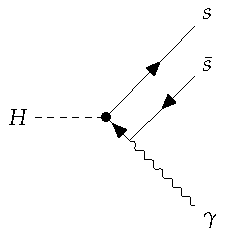
\includegraphics[height=0.26\mylength]{resources/H_rare_decays_vertices/v1.pdf}
            \setlength{\unitlength}{0.26\mylength}
            \caption{\footnotesize (a)}
    \end{subfigure}%
    \begin{subfigure}[t]{0.5\mylength}
            \centering
            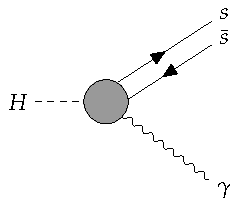
\includegraphics[height=0.26\mylength]{resources/H_rare_decays_vertices/v2_2.pdf}
            \setlength{\unitlength}{0.26\mylength}
            \caption{\footnotesize (b)}
    \end{subfigure}%
    \vspace*{-0.0cm}
    \caption{Direct (a) and indirect (b) contributions involved in the decays under analysis. Here we have considered the decay to a strange-antistrange quark pair, but it is analogous for the other light quarks.}
    \label{fig:Higgs_rare_decay_veritces}
    \vspace*{-0.0cm}
\end{figure}

According to the Standard Model, the direct contribution is of the order of $10^{-11}$, while the indirect contribution is of the order of $10^{-6}$, which means that higher-order corrections dominate the behaviour of these type of decays.

A few examples of diagrams that contribute to the effective vertex are provided in Figure \ref{fig:Higgs_decays_indirect}. In diagram (a) the blue loop can either be a heavy charged fermion loop or a $W^{\pm}$ boson loop.

\begin{figure}[!ht]
    \captionsetup[subfigure]{labelformat=empty}
    \vspace*{-0.2cm}
    \centering
    \setlength{\mylength}{\textwidth}
    \begin{subfigure}[t]{0.333\mylength}
            \centering
            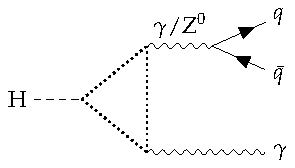
\includegraphics[width=0.323\mylength]{resources/H_rare_indirect/v1.pdf}%50x28
            \caption{\footnotesize (a)}
    \end{subfigure}%\begin{subfigure}[t]{0.5\mylength}
    \begin{subfigure}[t]{0.333\mylength}
            \centering
            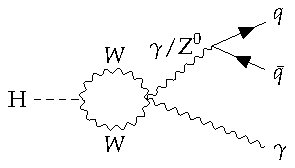
\includegraphics[width=0.323\mylength]{resources/H_rare_indirect/v2.pdf}%50x28
            \caption{\footnotesize (b)}
    \end{subfigure}%\begin{subfigure}[t]{0.5\mylength}
    \begin{subfigure}[t]{0.333\mylength}
            \centering
            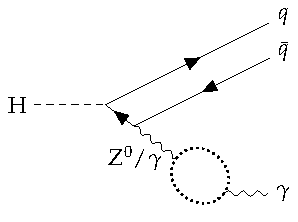
\includegraphics[width=0.323\mylength]{resources/H_rare_indirect/v4.pdf}%3:41x35 %4:50x37
            \caption{\footnotesize (c)}
    \end{subfigure}%\begin{subfigure}[t]{0.5\mylength}
    %\begin{subfigure}[t]{0.5\mylength}
    %        \centering
    %        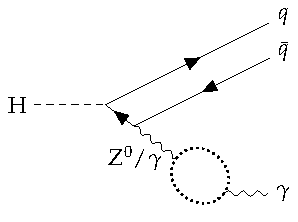
\includegraphics[height=0.26429\mylength]{resources/H_rare_indirect/v4.pdf}
    %        \caption{\footnotesize (d)}
    %\end{subfigure}%\begin{subfigure}[t]{0.5\mylength}
    %\vspace*{-0.0cm}
    \caption{Some examples of the many one-loop diagrams accounted for in the effective vertex. The blue loops are heavy charged fermion or $W^{\pm}$ boson loops.}
    \label{fig:Higgs_decays_indirect}
    \vspace*{-0.0cm}
\end{figure}

To ultimately compute the Yukawa couplings to the lighter families of quarks, one has to take into consideration contributions from both the direct and the indirect vertex, since experimentally what is measured from the direct decay is the overall effect coming from both vertices.

Therefore, the full diagrams of the decays that are object of study in these thesis (bottom half part of Table \ref{tab:Higgs_rare_decays}) are shown in Figure \ref{fig:Higgs_decays_studied}.

\begin{figure}[!ht]
    \captionsetup[subfigure]{labelformat=empty}
    \vspace*{-0.2cm}
    \centering
    \setlength{\mylength}{\textwidth}
    \begin{subfigure}[t]{0.43\mylength}
            \centering
            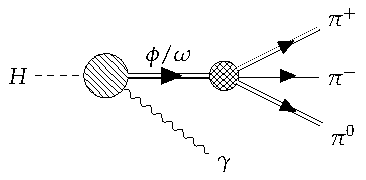
\includegraphics[width=0.41764\mylength]{resources/H_rare_decays_diagrams/v1.pdf}%62mm
            \caption{\footnotesize (a)}
    \end{subfigure}%\begin{subfigure}[t]{0.5\mylength}
    \begin{subfigure}[t]{0.57\mylength}
            \centering
            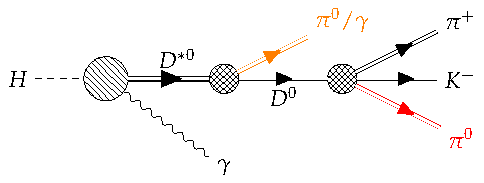
\includegraphics[width=0.55236\mylength]{resources/H_rare_decays_diagrams/v2_1.pdf}%82mm
            \caption{\footnotesize (b)}
    \end{subfigure}%\begin{subfigure}[t]{0.5\mylength}
    \caption{Full diagrams of the Higgs rare decays studied. Diagram (a) shows the decays $\text{H}\protect\decaysto \phi/\omega\gamma$. Diagram (b) shows the different decays $\text{H}\protect\decaysto D^{*0}\gamma$, where the orange line indicates that the particle can either be a $\pi^{0}$ ($\sim$ 65\%) or a $\gamma$ ($\sim$ 35\%) \cite{PDG}. This last diagram includes the two decays involving $D^{*0}$ studied, where $\pi^{0}$ is not there for the 2-body decay of the $D^{0}$ meson.}
    \label{fig:Higgs_decays_studied}
    \vspace*{-0.0cm}
\end{figure}

Diagram \ref{fig:Higgs_decays_studied} (a) depicts the decays $\text{H}\decaysto \phi\gamma$ and $\text{H}\decaysto \omega\gamma$, which are very similar and are going to share a lot of the features of the framework built. Diagram \ref{fig:Higgs_decays_studied} (b) shows the decays involving a $D^{*0}$ meson, $\text{H}\decaysto D^{*0}\gamma$, where the orange line from the decay of the $D^{*0}$ meson indicates that the particle can either be a $\pi^{0}$ (in around 65\% of the cases) or a $\gamma$ ($\sim$ 35\%) \cite{PDG}. This diagram encompasses the two decays involving $D^{*0}$ studied, where $D^{0}\decaysto K^{-}\pi^{+}$ corresponds to the diagram where the red line associated to $\pi^{0}$ is removed, and $D^{0}\decaysto K^{-}\pi^{+}\pi^{0}$ where the red edge is maintained. It is worth noting that these last decays are not charge symmetric because $D^{0}\decaysto K^{+}\pi^{-} (\pi^0)$ are doubly Cabbibo supressed (DC) \cite{PDG}. In the analysis we are only going to focus on the decays that are not DC suppressed, since it allows us to remove about half of background events.

The main difference between this analysis and the one studying the three decays presented in the top half of Table \ref{tab:Higgs_rare_decays} lies in the fact that we are dealing with 3-body decays involving neutral particles, which are more challenging to track compared to charged ones. That is why we will focus most of our attention on accurately recovering the missing neutral particles.

The main goal of this Master's Thesis is to compute a reasonable expected upper limit for the branching ratio of the aforementioned Higgs boson decays. Table \ref{tab:Higgs_rare_decays_values} shows the order of magnitude of the branching fractions one would ultimately like to measure. Nevertheless, due to the large hadronic background at the LHC, analyses of this kind are targeting an upper limit rather than a precise measurement at this stage.

Deviations from the predictions of the Standard Model within the Higgs boson sector can serve as compelling indications of new physics beyond our current understanding of particle physics. The Higgs boson plays a central role in the SM by giving particles mass through the Higgs mechanism. Therefore, any discrepancies in its properties, including decay widths, could reveal hidden phenomena and particles that the SM fails to describe.

One possible scenario involves determining an upper limit on a Higgs decay branching ratio that significantly exceeds the SM prediction. Such a discrepancy would suggest the presence of additional particles and interaction processes not accounted for in the SM. These new BSM particles could contribute to the Higgs decay width in ways not initially anticipated.

Accurate measurements are essential in this context, as they allow us to probe the Higgs sector with the highest level of precision. Through the precise determination of the Higgs boson's properties, one can identify even the most subtle deviations from the SM, providing clues about the nature of new physics. Consequently, the need for precision in Higgs boson measurements is of utmost importance, as it can not only further confirm the validity of the SM but also has the potential to illuminate the path towards a more comprehensive theory of particle physics, one that goes beyond the boundaries of the Standard Model.

The Future Circular Collider (FCC) project, with its proposed scenarios, including FCC-ee (electron-positron collisions) and FCC-hh (hadron-hadron collisions), presents a promising opportunity to advance our understanding of the Higgs boson and, by extension, the Standard Model \cite{FCC:2018byv}. The FCC-ee, with its high-energy lepton collisions, would enable us to conduct precise measurements of the Higgs boson's properties, including its interactions with other SM particles. This collider could provide an order of magnitude improvement in accuracy compared to current experiments, allowing for detailed studies of the Higgs, $W^\pm$, and $Z^0$ bosons, as well as the top quark \cite{Ellis:2015sca, dEnterria:2016fpc}. Together with the FCC-hh, which would operate with hadron collisions at significantly higher energies (potentially up to 30 times that of the current LHC \cite{FCC:2018vvp}), these colliders within the FCC project hold the potential to shed light on dark matter, probe neutrino masses, and investigate other unexplained phenomena.
